Multi-core processors consists of multiple CPUs or cores placed on a
single chip. Typically, each core is equipped with private level one
cache, other caches may or may not be shared between the cores
\cite{pacheco}. Each core is independent and the architecture is
categorized as a multiple instruction, multiple data (MIMD) system.
Processors and cores usually communicate implicitly via shared memory.

In a shared-memory system a collection of independent processors are
connected to a memory system via an interconnect network. There are
two principal types of shared-memory systems: uniform memory access
(UMA), and non-uniform memory access (NUMA). 

\section{Uniform memory access}

In UMA systems all processors are connected directly to main memory ,
see Figure \ref{fig:uma-arch}. Each core can access data from all of
the other cores directly. Access to all memory locations are the same
for each core. UMA systems main advantage in relation to NUMA systems
is their simplicity.

\begin{figure}[H]
	\centering
	% left bottom right top
	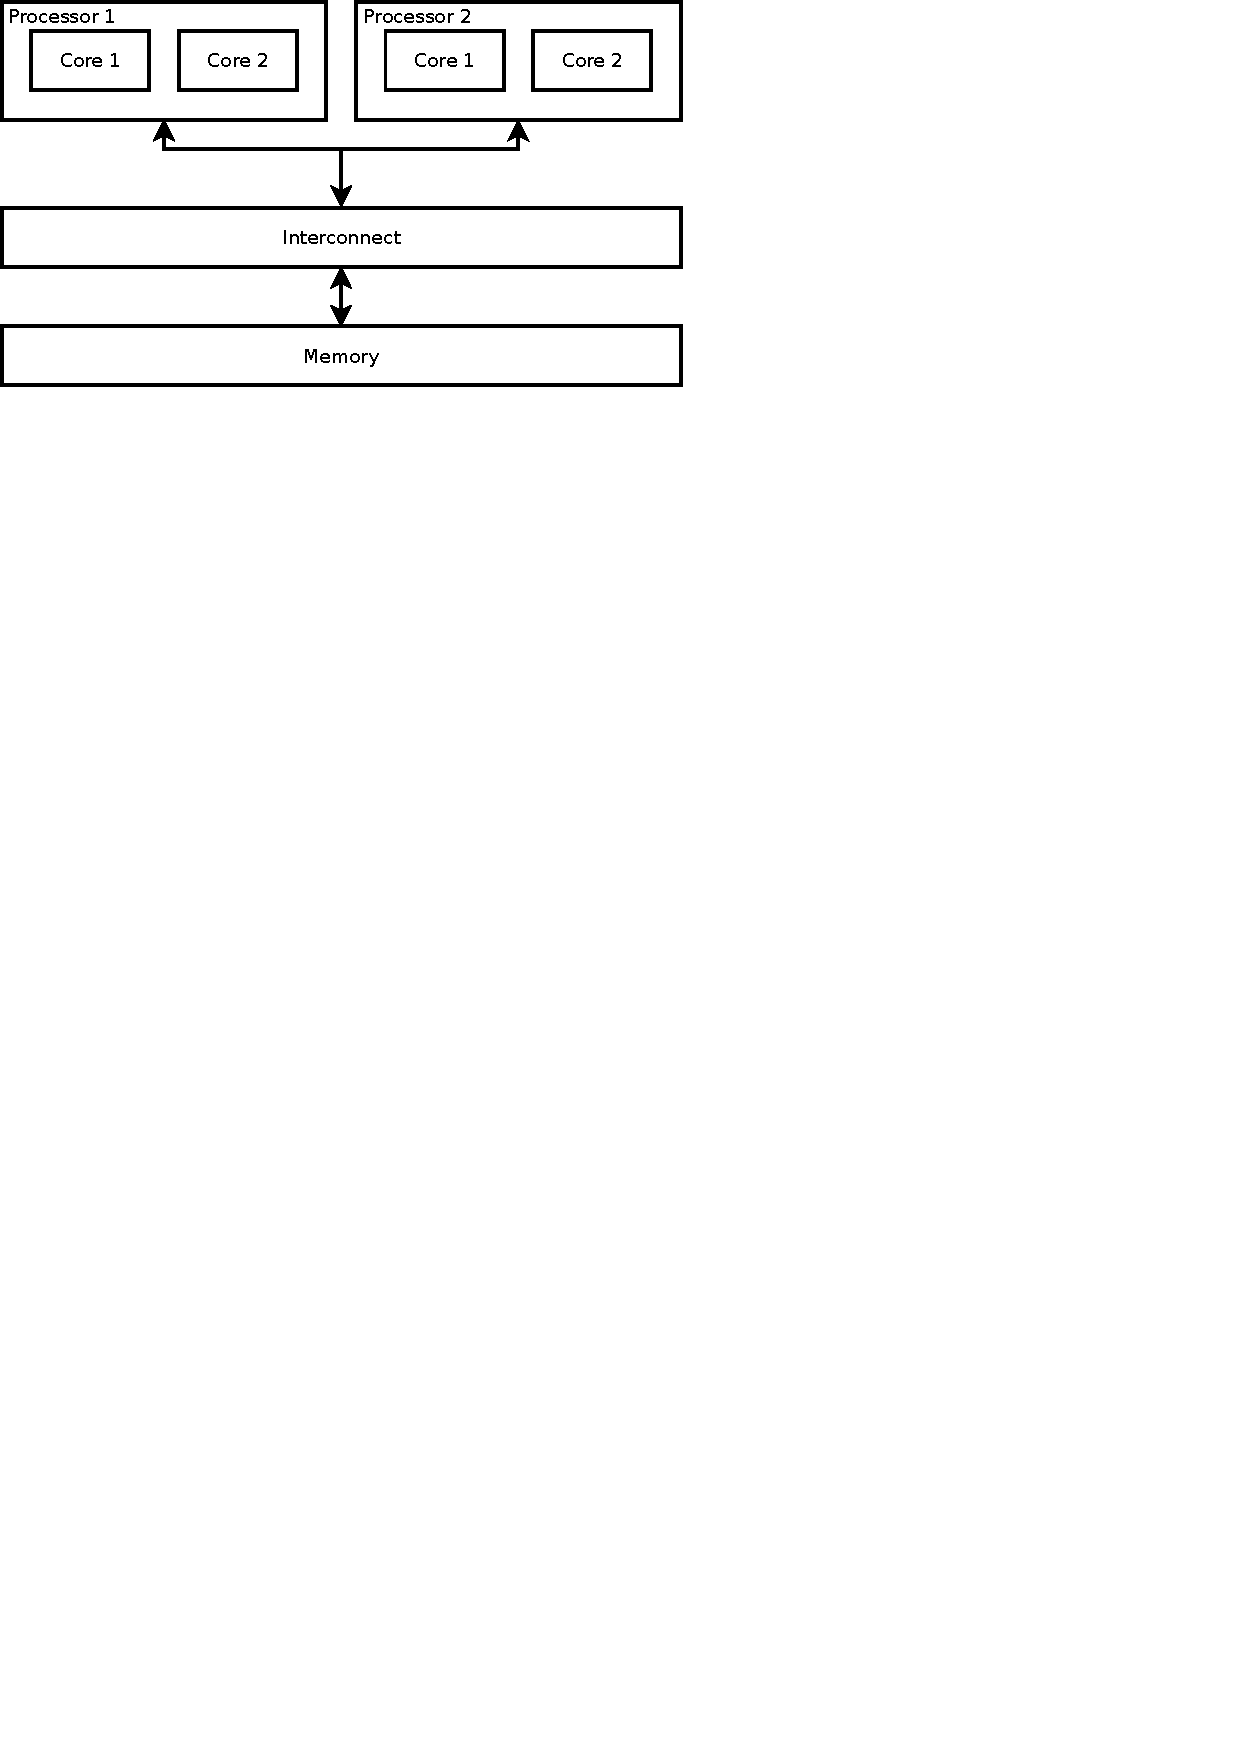
\includegraphics[scale=0.8,trim=0 23.15cm 9.4cm 0]{img/uma}
	\caption{UMA architecture}
	\label{fig:uma-arch}
\end{figure}

\section{Non-uniform memory access}

In NUMA systems each processor is directly connected to a block of
main memory, and the processors can reach each others data through
special hardware built into the processors, see Figure
\ref{fig:numa-arch}. A memory location that a processor is directly
connected to can be accessed faster than a memory location that must
be accessed through another chip \cite{pacheco}. Advantages of the
increased complexity is that the system can address a larger memory
space, and directly memory access typically is faster than in UMA
systems.

\begin{figure}[H]
	\centering
	% left bottom right top
	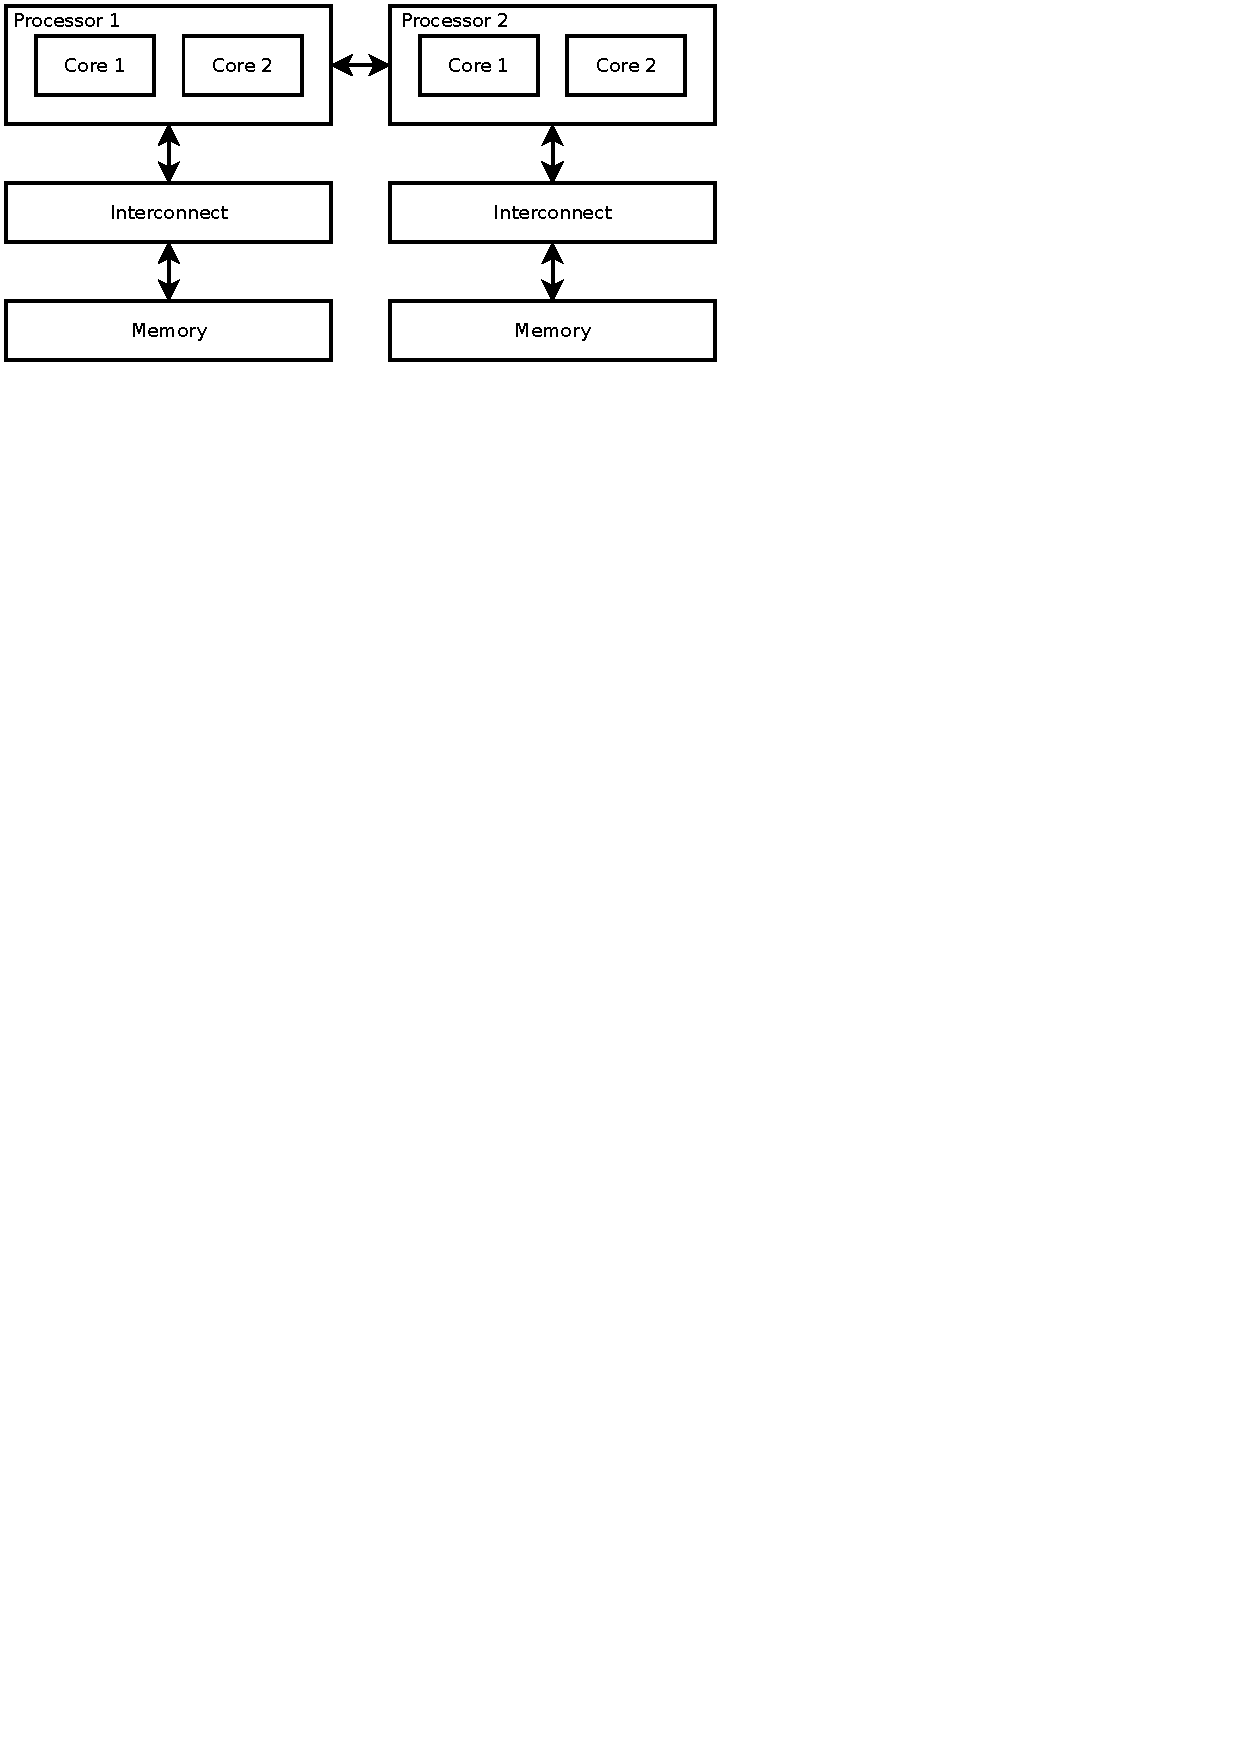
\includegraphics[scale=0.8,trim=0 23.55cm 8.8cm 0]{img/numa}
	\caption{NUMA architecture}
	\label{fig:numa-arch}
\end{figure}

\section{Cache hierarchy}
\label{sec:cache-hierarchy}

Each core in a multi-core processor typically have a private level 1
cache (L1). In the Intel Nehalem family, each core contains an
instruction cache, a first level data cache and a second-level unified
cache (L2). Furthermore, each physical processor includes a third
level cache (L3) shared by all cores in the processor. L1 and L2 are
writeback and non-inclusive, L3 is writeback and inclusive so that a
cache line that exists in any other level is also included in L3. An
advantage of using L3 this way is that snoop traffic between
processors can be reduced.  \cite{inteloptimization}. Table
\ref{tab:cache-hierarchy} shows data cache parameters for the Intel
Core i7 processor, a member of the Nehalem family, with 4 physical
cores.

\begin{table}[H]
	\centering
	\begin{tabular}{|l|l|l|l|}
		\hline
		Level & Capacity & Access latency (clocks)  \\
		\hline \hline
		L1 & 32KB & 4 \\ \hline
		L2 & 256KB & 10 \\ \hline
		L3 & 8MB & 35-40 \\ \hline
	\end{tabular}
	\caption{Cache parameters of Intel Core i7 Processors}
	\label{tab:cache-hierarchy}
\end{table}

\section{Multithreading}

Multithreaded processors concurrently executes instructions from
different threads of control within a single pipeline. These can be
placed in two basic categories: temporal multithreaded processors and
simultaneous multithreading (SMT) processors. Temporal multithreaded
processors issues instructions from a single thread every clock cycle
while SMT processors issue instructions from multiple threads in the
same cycle \cite{crayxmt}.

Hyper-threading, Intels implementation of SMT, maps one physical core
into two logical cores by decoding instruction streams in alternate
cycles. The operating system sees each logical core as one processor.
The main purpose of Hyper-threading is to decrease the number of
dependent instructions in the pipeline. Logical threads executed on
one core shares most of their cache/execution resources
\cite{inteloptimization}.

\section{Threads and processes}

Threads and processes are both methods of parallelizing an
application.  However, processes are independent execution units that
contain their own state information, use their own address spaces, and
only interact with each other via interprocess communication
mechanisms. Processes are typically used in parallel database systems,
where message passing is a common means of communication. 

In contract, threads share the same state and memory space. They are
not independent in the same way as a process, but can still be
executed concurrently so that parallel compute power is exploited.
One process can start multiple threads. Additionally, threads use a
simple and fast method of communication, shared memory. Typically, all
threads in an application can access a set of shared variables in
exactly the same way as private variables are accessed. However,
developers must take additional care to avoid race conditions.
Accessing the same variable from multiple threads are normally
accompanied by locks (mutexes), or atomic operations.

Arguments for using threads instead of processes are that they are
cheaper to create, and have a simple and fast model of communication.
However, processes often used as a means of isolating tasks for
security reasons, and when tasks are inherently independent. Threads
incur an increased risk of race conditions compared to processes.

\section{Programming frameworks}

This section contains an overview of selected shared-memory
programming frameworks and libraries. Advantages and disadvantages are
noted for each framework. Data from this section are used to choose a
suitable framework for implementation in Chapter
\ref{chap:implementation-and-evaluation}.

\subsection{Pthreads}

Pthreads is short for POSIX threads and specifies a low-level
application programming interface (API) for multithreaded programming
in Unix-like operating systems. It is implemented as a C library and
is widely used in both real-life implementations and research papers.

\paragraph{Thread distribution} Programmers can create an arbitrary
number of threads using the function pthread\_create. The operating
system (OS) is responsible for distribution threads among cores.
Pthreads use the fork-join paradigm, where all threads spawn from a
master thread and are joined back to one thread before program
termination (using pthread\_join).

\paragraph{Memory sharing} Memory sharing is achieved by giving all threads access to global
variables, and keeping local variables private for the thread
executing the function \cite{pacheco}. It is possible to pass pointers
to pthread\_create, typically used to give each thread a unique id and
working set.

\paragraph{Synchronization}
Pthreads include mutexes, read-write locks, conditional variables, and
barriers for synchronization. In more involved cases semaphores can be
used (not included in the pthread definition, but provided in by
semaphores.h)

\subsection{OpenMP}

OpenMP is a mature and widely used API for shared memory parallel
programming. Code is parallelized using compiler directives and C
code. Programmers define areas that can be executed in parallel and
OpenMP handles the threading \cite{pacheco}. This framework is more
high-level than Pthreads, it aims make the creation of large-scale
high-performance programs easier. OpenMP was explicitly designed to
allow programmers to incrementally parallelize existing serial
programs. It is best equipped with pragmas for loop-level parallelism,
typically found in compute intensive workloads. For more general
workloads, the simplicity may be counter-productive.

\paragraph{Thread distribution} OpenMP allows programmers to give the
compiler hits about code sections that can be run in parallel using
pre-compiler directives (pragmas). Number of threads started is system
dependent, but most systems will start one thread per core.
Programmers can explicitly set number of threads that should be
started using an environment variable (OMP\_NUM\_THREADS), or a
function call. However, allowing OpenMP to handle thread count is
normally the best solution. A classical example is OpenMPs pragma for
loops, this will automatically partition data and execute loop in
parallel. OpenMP also have more complex (or specific) directives like
simd, that indicates that data parallelism can be utilized.

\paragraph{Memory sharing} Each OpenMP thread can use shared, and
private memory. By default, shared variables are determined by static
scope, as in sequential C code. For more fine-grained control OpenMP
allows programmers to define variables that should be regarded as
thread private or shared. It is common to define all variables as
private by a call to default(none), and specify all shared variables
explicitly using the shared directive. If a private variable is
declared outside the parallel region, OpenMP generates one copy for
each thread.

\paragraph{Synchronization} Synchronization is achieved by defining
critical sections, each section can be named for fine-grained control.
In some cases the atomic directive can be used to increase
performance, this directive is designed to exploit special hardware
instructions. For reduction operators (sum, product, etc.) OpenMP
provides a reduction clause. In addition, simple locks, and barriers
are provided. \cite{pacheco}

\subsection{Cilk++}

Cilk++ is a commercial version of the Cilk language developed at the
MIT for multithreaded parallel programming. It is an extension to the
C++ language adding three basic keywords to process loops in parallel,
launch new tasks, and synchronize between tasks
\cite{multicorecomparison}. Intel, the owner of Cilk++, claims that
the runtime system operates smoothly on systems with hundreds of
cores. Cilk++ has features similar to OpenMP.

\paragraph{Thread distribution} Cilk++ use an efficient work-stealing
scheduler to automatically distribute tasks among available cores.
Tasks can either be implemented as separate functions or in iterations
of a loop. The keyword \_Clik\_spawn are used to modify a function
call to tell the runtime system that the function may run in parallel.
There is also a keyword equivalent to OpenMPs loop pragma that
automatically run a for-loop in parallel.

\paragraph{Memory sharing} Memory is shared similar to OpenMP, but
Cilk++ introduces a new concept, hyperobjects. Hyperobjects enables
many parallel threads to coordinate updating of a shared variable in
the form of reducers, holders and splitters. Each thread have its own
unique view of a reducer.

\paragraph{Synchronization} The keyword \_Cilk\_sync can be used to
indicate that the current function can not continue past a certain
point in parallel with its spawned children. Additionally, Cilk++
provides reduction operators to allow threads to access nonlocal
variables safely. Locks can be implemented in various ways, for
instance, pthread mutexes can be used directly.

\subsection{UPC}

Unified Parallel C (UPC) is an extension of the C programming language
designed for high performance computing on large-scale parallel
machines. The language provides a uniform programming model for both
shared and distributed memory hardware \cite{upc}. UPC is actively
developed at Berkley, latest version released in 2012.

\paragraph{Thread distribution} UPC uses a Single Program Multiple
Data (SPMD) model of computation in which the amount of parallelism is
fixed at program startup time, typically with a single thread of
execution per processor. Number of threads can be changed using a
variable named THREADS.

\paragraph{Memory sharing} The programmer is presented with a single
shared, partitioned address space, where variables may be directly
read and written by any thread. Each thread can use a combination of
shared and private data. By default, data is considered private, data
can be shared using a C type-qualifier.

\paragraph{Synchronization} Thread interaction is explicitly managed
by the programmer through primitives provided by the language.  UPC
includes locks, barriers and memory fences.

\subsection{SWARM}

SWARM is short for "SoftWare and Algorithms Running on Multicore". It
is a open source programming framework for multi-core hardware. SWARM
is built on POSIX threads and allows developers access to low-level
functionality as well as high-level constructs for more convenient
parallelization \cite{swarm}.

\paragraph{Thread distribution} Threads can be distributed by defining
functions as tasks that can be run in parallel, or by using loop
parallelism similar to OpenMP. Several basic loop parallelization
directives are included to implicitly partition loops among cores and
so that they can be executed in parallel. Both block and cyclic
partitioning interfaces are supported.

\paragraph{Memory sharing} SWARM provides directives, to dynamically
allocate and release shared data structures. For thread private
variables, a replication primitive is provided to create a unique copy
for each core.

\paragraph{Synchronization} Common synchronization primitives like
barrier and reduce are provided. In addition pthread mutexes can be
used to implement locks.

\subsection{Phoenix MapReduce}

Phoenix is a shared-memory implementation of Google's MapReduce model
for data-intensive processing tasks \cite{mapreduce}. Phoenix can be
used to program multi-core chips as well as shared-memory
multiprocessors. The framework is developed at Standford
University, latest update was released in 2011. The current
implementation provides an API for C and C++.

\paragraph{Thread distribution} The user specifies the algorithm using
two functions, map and reduce. The map function processes the input
data and generates a set of intermediate key/value-pairs. The reduce
function merges the intermediate values which have the same key.
Phoenix use threads to spawn parallel map and reduce tasks. Tasks are
dynamically scheduled across available processors (or cores) in order
to achieve balanced load and to maximize throughput.

\paragraph{Memory sharing} Shared-memory buffers are used to
facilitate communication without excessive data copying. However, the
MapReduce paradigm is best suited for independent tasks that can be
merged at the end with minimal data sharing.

\paragraph{Synchronization} The MapReduce paradigm does not provide
explicit synchronization constructs. Synchronization is implicitly
performed in the reduce operation. As a consequence, MapReduce is not
a very general method for shared-memory programming.

\subsection{Intel TBB}

Intel Threading Building Blocks (TBB) is a commercial library that
aims to help developers leverage multi-core performance without being
threading experts \cite{tbbarticle}.  This library allows developers
to program multi-core processors in a high-level view using tasks. It
can coexist with other multi-core libraries, like pthreads \cite{tbb}.
TBB emphasize scalable, data parallel programming, enabling multiple
threads to work on different parts of a collection. According to Intel
TBB is a widely used C++ template library for task parallelism.

\paragraph{Thread distribution} Developers specify tasks that are
automatically mapped to threads in an efficient manner. TBB supports
nested parallelism, making it possible to build larger parallel
components by combining smaller parallel components. Loops can be
parallelized by moving the loop body into a functor (C++ objects that
can are treated as a function) and passing the functor in a library
call.

\paragraph{Memory sharing} TBB provides two memory allocator templates
designed to improve scalability and avoid false sharing. Two objects
allocated by cache\_aligned\_allocator are guaranteed to not have
false sharing. For memory sharing, TBB provides concurrent containers
with fine-grained locking and lock-free techniques. 

\paragraph{Synchronization} Mutual exclusion is implemented by mutexes
and locks. TBB supports a number of synchronization constructs, like
spin\_mutex, scoped\_lock, and recursive and non-recursive mutexes.
There is also support for atomic operations using template functions.

\subsection{Comparison}

Table \ref{tab:comparison} give an overview of frameworks previously
discussed. Compiler- and language support is based on data from recent
articles and information posted on the official web sites for each
framework.

\begin{table}[H]
	\centering
	\begin{tabular}{|p{2cm}|p{1.6cm}|p{1.7cm}|p{2.2cm}|p{2.5cm}|p{2cm}|}
		\hline
		Name & 
			Language support & 
			Compiler support \footnotemark & 
			API type & 
			Recommended parallelization & 
			Notable features \\
		\hline \hline
		OpenMP & 
			C, C++, Fortran & 
			Good & 
			Compiler directives &
			task or data & 
			\\ \hline
		Cilk++ (Intel) & 
			C++ & 
			Average & 
			C++ keywords and hyperobjects &
			task or data & 
			Race detector, Performance analyzer \\ \hline
		TBB (Intel) & 
			C++ & 
			Good & 
			Special C++ objects (lambda functions available in a few compilers) &
			task or data & 
			Concurrent container classes (hash maps, vectors and queues) \\ \hline
		Pthreads &
			C &
			Good &
			types and procedure calls &
			task &
			\\ \hline
		SWARM &
			C &
			Good &
			types and procedure calls &
			task &
			\\ \hline
		UPC &
			C &
			Average &
			keywords, types, procedure calls, and expressions &
			task or data &
			\\ \hline
		Phoenix++ &
			C++ &
			Good &
			C++ templates &
			map-reduce &
			\\ \hline

	\end{tabular}
	\caption{Feature comparison between multi-core frameworks}
	\label{tab:comparison}
\end{table}

\footnotetext{Good: All major compilers. Average: At least one
open source compiler. Poor: Only Proprietary compilers.}

\section{Code optimization}
\label{sec:optimization}

In shared-memory programming it is important to consider common
bottlenecks to achieve an acceptable performance. If algorithms are
parallelized without careful planning, they can easily become slower
than sequential versions due to less optimal memory access patterns,
synchronization, thread creation costs, or false sharing. It is
essential to avoid false sharing and minimize time in critical
sections.

False sharing is a performance degrading access pattern that can occur
in systems with concurrent caches. It is encountered if a thread
periodically access data that never will be altered by another party
and this data is placed in the same cache block as data that is
altered. There are different methods to handle this. An obvious method
is to partition data so that such a situation will never occur. If
this is not possible, data structures can be padded so that they fit
in an entire cache line, making it impossible for data structures used
by other threads to be placed in the same block.

Critical sections are sections in the code that require sequential
execution, i.e. are unable to exploit parallelism. In some cases
critical sections must be used to avoid race conditions. Programmers
typically need to place results in a shared data structure. Insertions
and reads from this structure in normally have to to be synchronized
to ensure data consistency. It is normally not a good idea to lock the
entire structure, as this will induce a big sequential section, rather
fine-grained locking should be used so that multiple threads can work
on the same structure concurrently. This is closely related to Amdahls
law: $\frac{1}{(1-P)+\frac{P}{S}}$, where P is parallel part and S is
sequential part. Speedup is limited by the sequential fraction of the
program. Fine-grained locking can in many cases be used to reduce the
sequential fraction can be reduced.

Obviously, shared-memory algorithms will take advantage of traditional
optimization techniques as well. Therefore, efforts should be made to
improve cache locality and sequential memory access. General purpose
processors are best suited for sequential memory access, and have
efficient cache hierarchies that can be exploited to improve algorithm
performance. However, the authors of \cite{hashjoin} note that modern
processors are very effective in hiding cache miss latencies through
multi-threading. Therefore computation and synchronization costs can
be just as important when shared-memory algorithms.

Techniques for Non-uniform memory access (NUMA) are evaluated in
\cite{sortmergejoin}. This article states that sequential scans of
non-local memory heavily profit from pre-fetching and cache locality.
Based on micro-benchmarks on NUMA-affine versus NUMA-agnostic data
processing, authors define three basic rules for NUMA-affine scalable
multi-core parallelization:

\begin{description}
	\item[C1] Avoid random writes to non-local memory locations
	\item[C2] If remote reads are necessary, use a sequential access pattern
	\item[C3] Avoid waiting for other nodes
\end{description}

In conclusion, algorithms should be cache-concious, use sequential
memory access, avoid false sharing and spend minimal time in critical
sections. Data structures can have a major impact on performance, both
for sequential and parallel algorithms. Concurrent data structures
will in many cases take advantage of fine-grained locking
mechanisms to allow multiple threads to access different regions
at the same time. 
